%%%%%%%%%%%%%%%%%%%%%%%%%%%%%%%%%%%%%%%%%
% Beamer Presentation
% LaTeX Template
% Version 1.0 (10/11/12)
%
% This template has been downloaded from:
% http://www.LaTeXTemplates.com
%
% License:
% CC BY-NC-SA 3.0 (http://creativecommons.org/licenses/by-nc-sa/3.0/)
%
%%%%%%%%%%%%%%%%%%%%%%%%%%%%%%%%%%%%%%%%%

%----------------------------------------------------------------------------------------
%	PACKAGES AND THEMES
%----------------------------------------------------------------------------------------

\documentclass{beamer}

\mode<presentation> {



% The Beamer class comes with a number of default slide themes
% which change the colors and layouts of slides. Below this is a list
% of all the themes, uncomment each in turn to see what they look like.

%\usetheme{default}
\usetheme{AnnArbor}
%\usetheme{Antibes}
%\usetheme{Bergen}
%\usetheme{Berkeley}
%\usetheme{Berlin}
%\usetheme{Boadilla}
%\usetheme{CambridgeUS}
%\usetheme{Copenhagen}
%\usetheme{Darmstadt}
%\usetheme{Dresden}
%\usetheme{Frankfurt}
%\usetheme{Goettingen}
%\usetheme{Hannover}
%\usetheme{Ilmenau}
%\usetheme{JuanLesPins}
%\usetheme{Luebeck}
% \usetheme{Madrid}
%\usetheme{Malmoe}
%\usetheme{Marburg}
%\usetheme{Montpellier}
%\usetheme{PaloAlto}
%\usetheme{Pittsburgh}
%\usetheme{Rochester}
%\usetheme{Singapore}
%\usetheme{Szeged}
%\usetheme{Warsaw}

% As well as themes, the Beamer class has a number of color themes
% for any slide theme. Uncomment each of these in turn to see how it
% changes the colors of your current slide theme.

%\usecolortheme{albatross}
\usecolortheme{beaver}
%\usecolortheme{beetle}
%\usecolortheme{crane}
%\usecolortheme{dolphin}
%\usecolortheme{dove}
%\usecolortheme{fly}
%\usecolortheme{lily}
%\usecolortheme{orchid}
%\usecolortheme{rose}
%\usecolortheme{seagull}
%\usecolortheme{seahorse}
%\usecolortheme{whale}
%\usecolortheme{wolverine}

%\setbeamertemplate{footline} % To remove the footer line in all slides uncomment this line
%\setbeamertemplate{footline}[page number] % To replace the footer line in all slides with a simple slide count uncomment this line

%\setbeamertemplate{navigation symbols}{} % To remove the navigation symbols from the bottom of all slides uncomment this line
}

\usepackage{graphicx} % Allows including images
\usepackage{booktabs} % Allows the use of \toprule, \midrule and \bottomrule in tables
\usepackage{booktabs}% http://ctan.org/pkg/booktabs
\usepackage{caption}
%----------------------------------------------------------------------------------------
%	TITLE PAGE
%----------------------------------------------------------------------------------------

\title[Photometric Redshifts]{Estimating the Photometric Redshifts of Galaxies Using Regression Techniques} % The short title appears at the bottom of every slide, the full title is only on the title page

\author[Momtaz, Salimi, Shakeri]{ A. Momtaz, M. H. Salimi, S.Shakeri}
%\rel{ Supervised by: P. Sahebsara, PhD.} % Your name
\institute[IUT] % Your institution as it will appear on the bottom of every slide, may be shorthand to save space
{
Department of Physics, Isfahan University of Technology, Isfahan 84156-8311, Iran. \\ % Your institution for the title page
\medskip
\textit{aidinmomtaz@ph.iut.ac.ir\\mhsalimi@ph.iut.ac.ir\\s.shakeri@iut.ac.ir} % Your email address
}
\date{July 7, 2021} % Date, can be changed to a custom date
\setbeamertemplate{caption}[numbered]
\begin{document}

\begin{frame}
\titlepage % Print the title page as the first slide
\end{frame}
%---------------------

%-----------------------

\begin{frame}
\frametitle{Overview} % Table of contents slide, comment this block out to remove it
\tableofcontents % Throughout your presentation, if you choose to use \section{} and \subsection{} commands, these will automatically be printed on this slide as an overview of your presentation
\end{frame}

%----------------------------------------------------------------------------------------
%	PRESENTATION SLIDES
%----------------------------------------------------------------------------------------
%----------------------------------------------------------------------------------------
%   Introduction
%----------------------------------------------------------------------------------------
\section{Introduction}
\subsection{Motivation}
\begin{frame}
 	\frametitle{Astronomical Surveys, SDSS}
    \begin{columns}[onlytextwidth]
    \begin{column}{.45\textwidth}
        \begin{figure}
            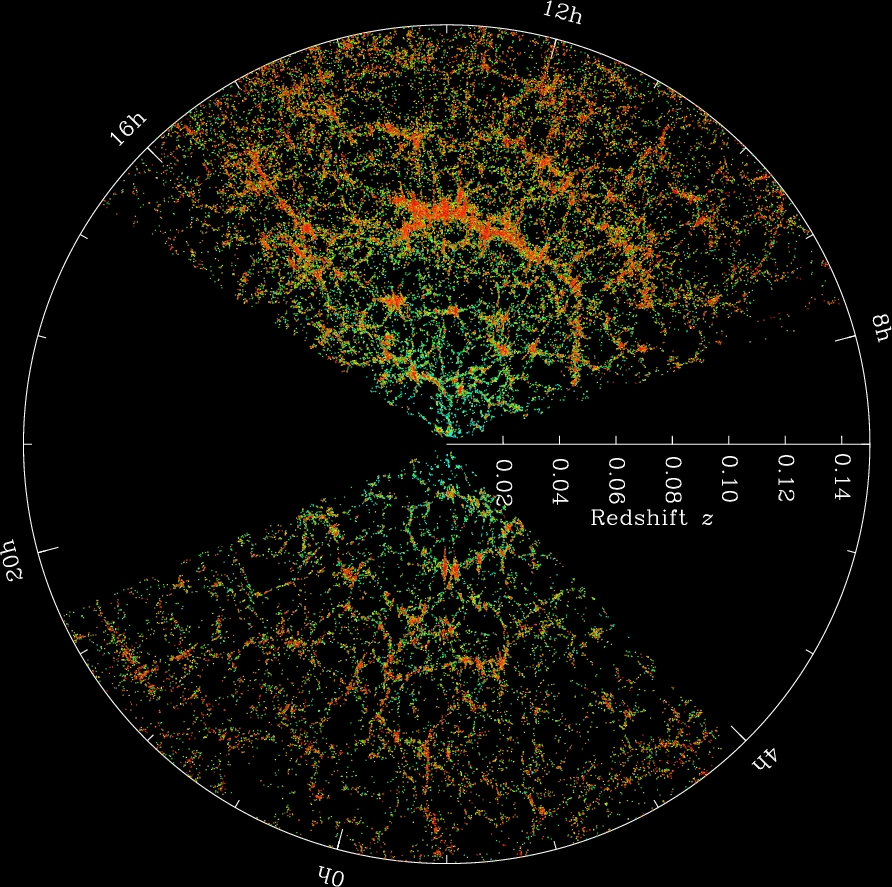
\includegraphics[width=\textwidth]{img/sdss_galaxy_map.jpg}
            \caption*{SDSS Galaxy Map}
        \end{figure}
    \end{column}
    \hfill
    \begin{column}{.45\textwidth}
    \begin{itemize}
        \item Galactic Archaeology
        \item Gas in the Galaxy
        \item Star Forming Regions
        \item Multi-Star and Planetary Systems
        \item White Dwarfs
    \end{itemize}
    \end{column}
    \end{columns}
    \end{frame}
\subsection{Spectroscopic and Photometric Redshifts}
\begin{frame}
	\frametitle{Measuring Redshift from Spectroscopy}
    \begin{figure}
        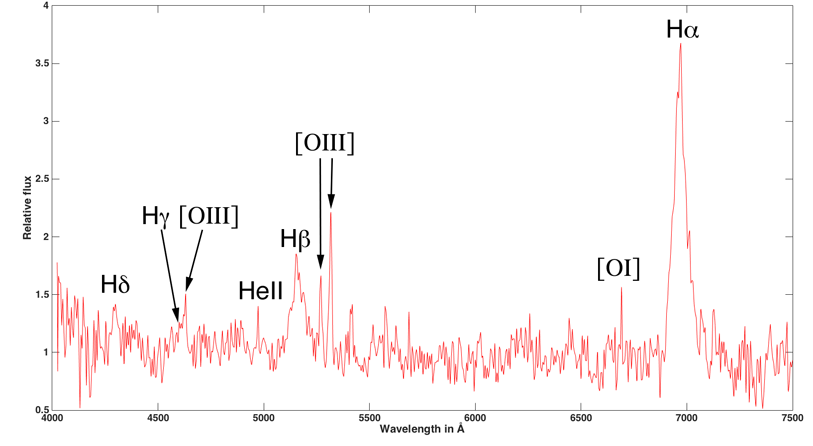
\includegraphics[scale=0.35]{img/Spectrum.png}
    \end{figure}
    \begin{equation}
        \lambda_{obs} = (1+z)\lambda_{em}
    \end{equation}
    \end{frame}
\begin{frame}
    \begin{figure}
	\frametitle{Measuring Redshift from Photometry}
        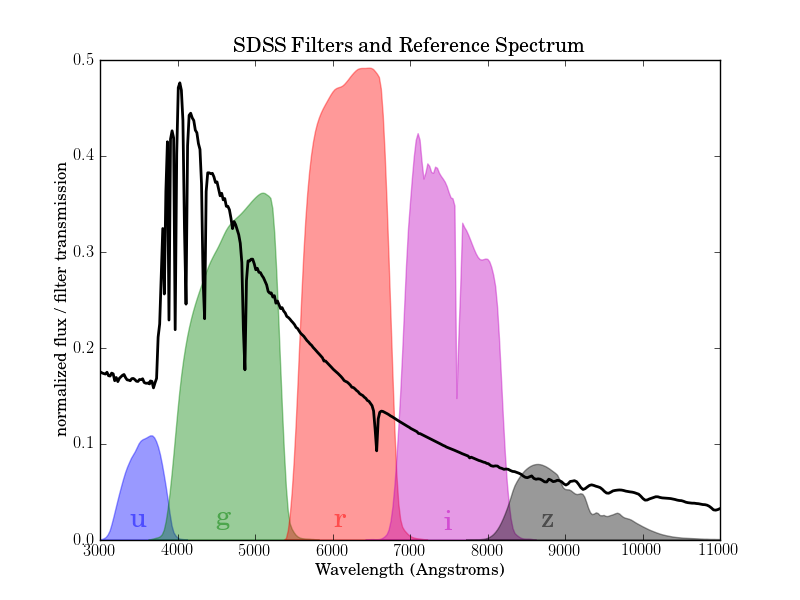
\includegraphics[scale=0.25]{img/sdss_plot.png}
    \end{figure}
    \begin{equation}
        u=m_{\text {ref }}-2.5 \log {10}\left[\int_{0}^{\infty} F(\lambda) S(\lambda) d \lambda\right]
    \end{equation}
    \end{frame}
\subsection{Machine Learning}
\begin{frame}
	\frametitle{Regression Algorithms}
    \begin{description}
        \item[Decision Tree] \hfill \\ Decision trees map a set of input features to their corresponding output targets. This is done through a series of individual decisions where each decision represents a node (or branching) of the tree. 
        \\[0.2in]
        \pause
        \item[Random Forest] \hfill \\ Random forests are an ensemble learning method for classification, regression and other tasks that operates by constructing a multitude of decision trees at training time. 
    \end{description}
    \end{frame}
\begin{frame}
	\frametitle{How does Decision Tree work?}
    \begin{figure}
        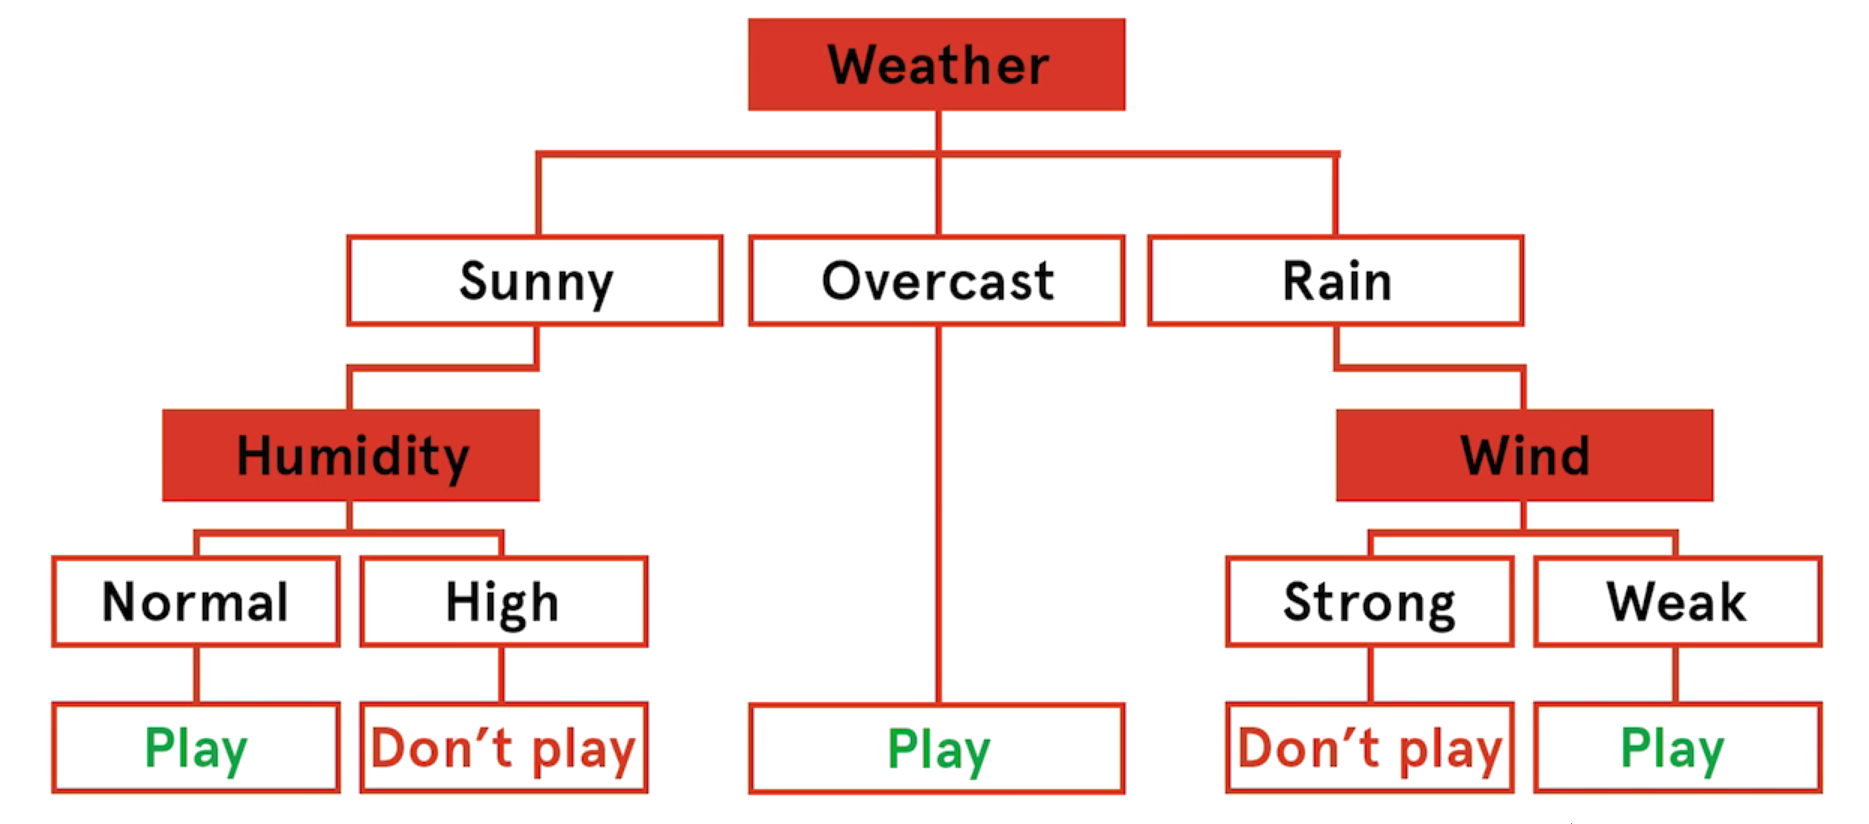
\includegraphics[scale=0.15]{img/decision_tree2.png}
        \caption*{Schematic View of Decision Tree}
    \end{figure}
    \end{frame}

\begin{frame}
	\frametitle{How does Random Forest work?}
    \begin{figure}
        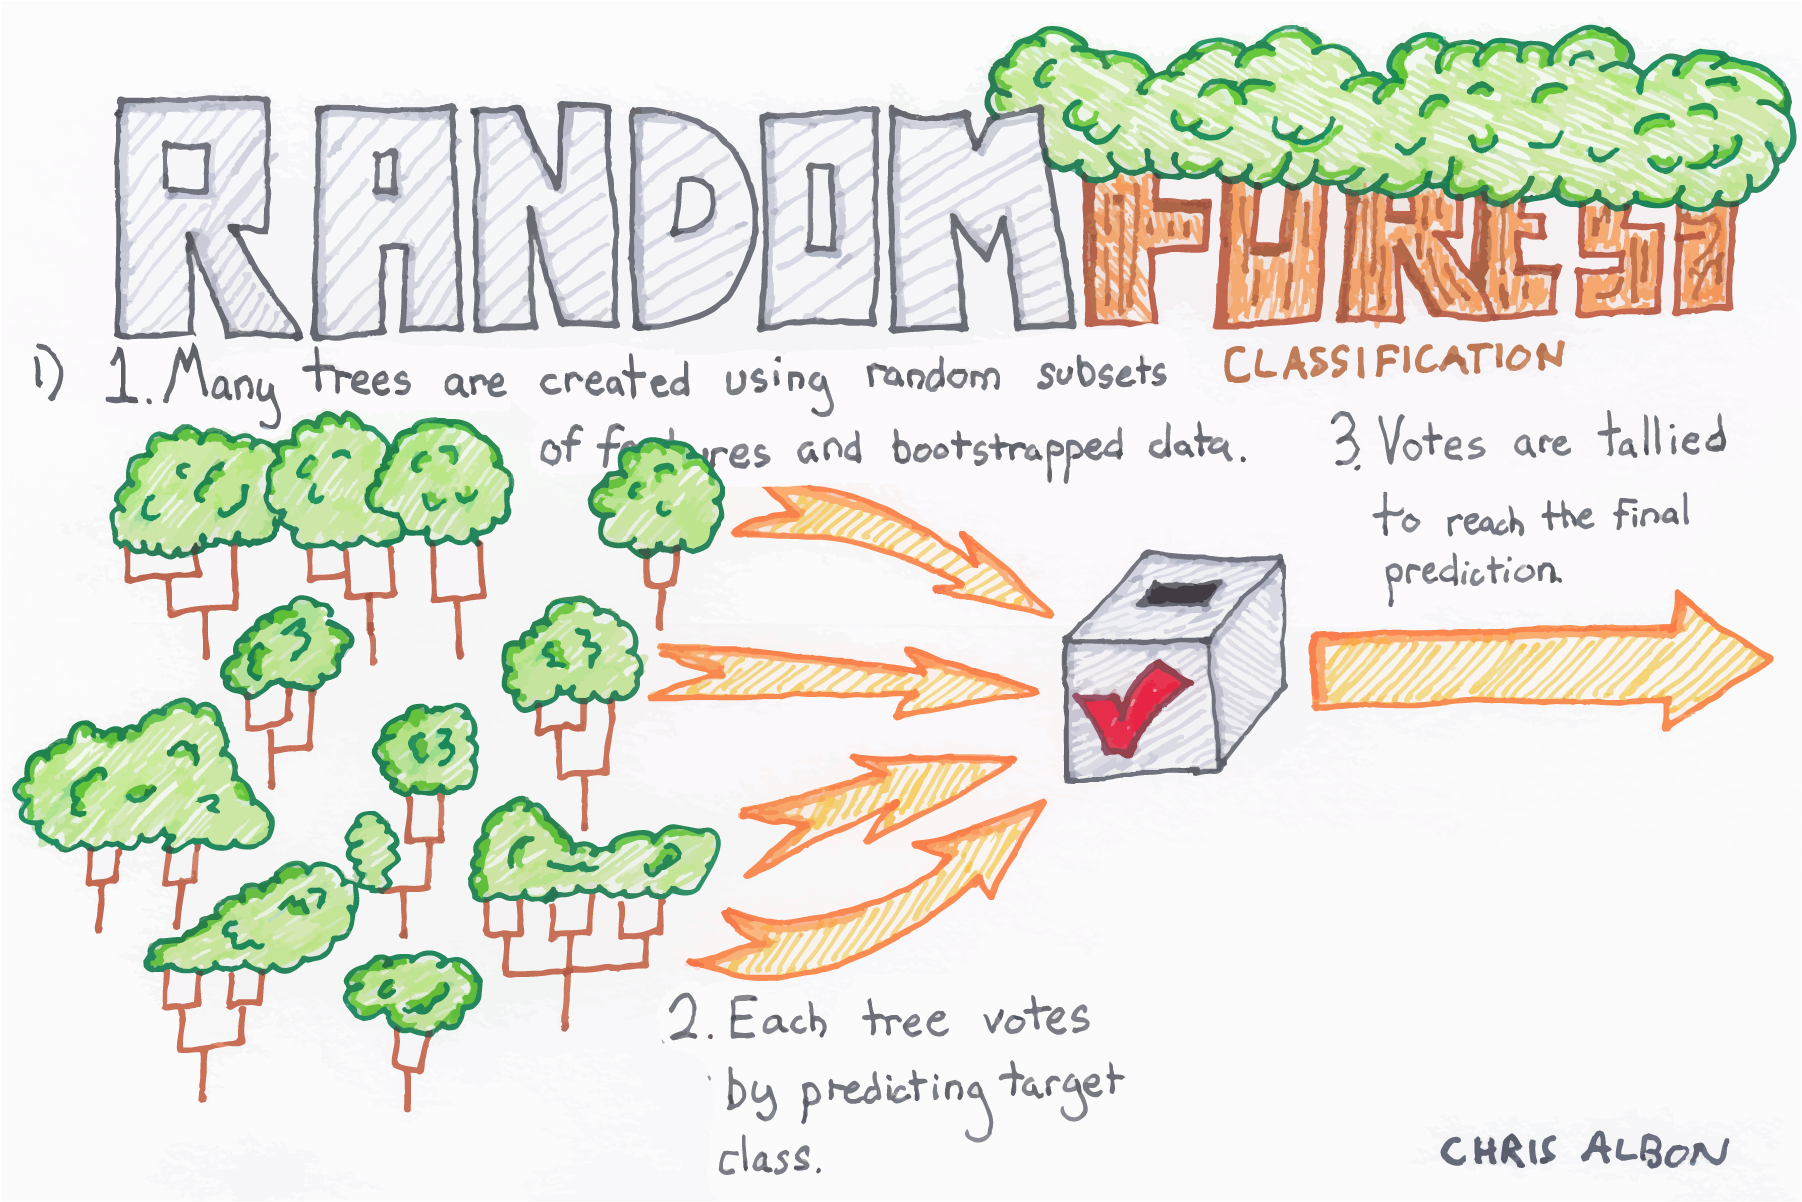
\includegraphics[scale=0.15]{img/Random_Forest.png}
        \caption*{Schematic View of Random Forest}
    \end{figure}
    \end{frame}
\begin{frame}
	\frametitle{Geometrical View of  Algorithm}
    \begin{figure}
        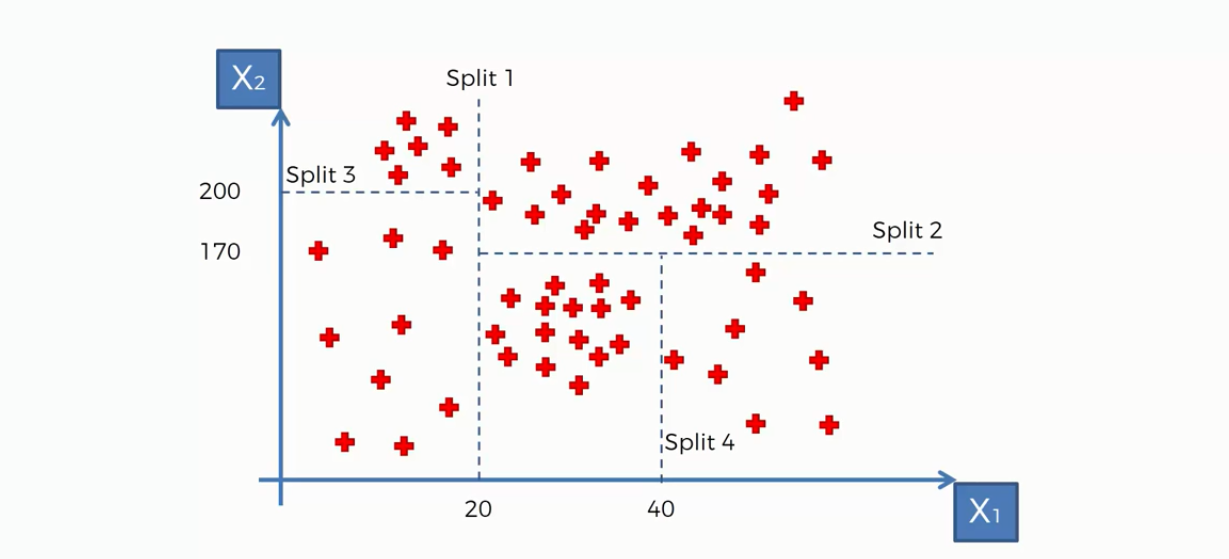
\includegraphics[scale=0.35]{img/decision_tree_intuition.png}
        \caption*{Desicion Tree Intuition}
    \end{figure}
    \end{frame}
%----------------------------------------------------------------------------------------
%   Literature Survey
%----------------------------------------------------------------------------------------
\section{Literature Survey}
\begin{frame}
        \frametitle{ANN}
        \begin{figure}
            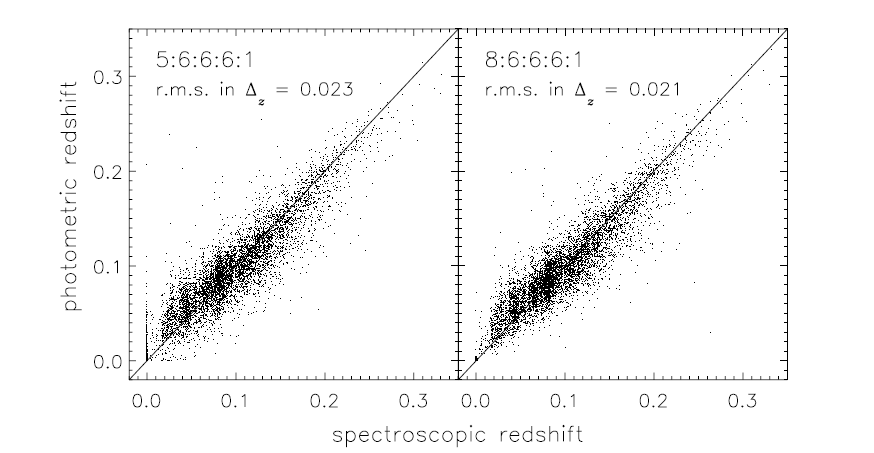
\includegraphics[scale=0.3]{img/lit_survay.png}
            \caption*{ugriz Photometry}
        \end{figure}
        \begin{itemize}
            \item Sample Size: 20000 Galaxies
            \item Testing Set: 7000 Galaxies
        \end{itemize}
        \end{frame}
%----------------------------------------------------------------------------------------
%   Methodology
%----------------------------------------------------------------------------------------
\section{Methodology}
\subsection{Data Preprocessing}
\begin{frame}
	\frametitle{Preparing the Dataset}
    \begin{figure}
	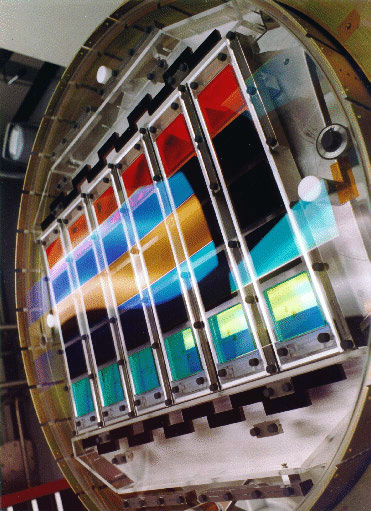
\includegraphics[scale=0.2]{img/SDSS_imaging_camera.jpg}
	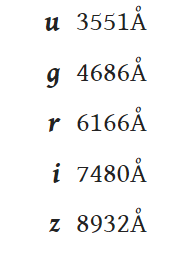
\includegraphics[scale=0.5]{img/wavelengths.png}
        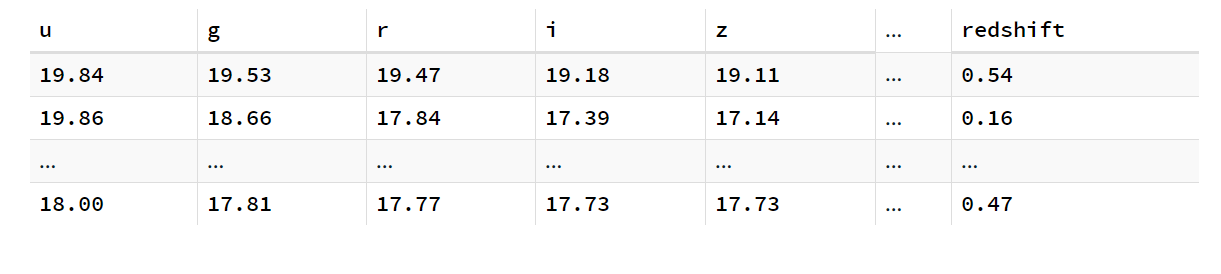
\includegraphics[scale=0.3]{img/sdss_data.png}
        \caption*{SDSS Data Sample}
    \end{figure}
    \end{frame}
\begin{frame}
	\frametitle{Contour map of the redshifts}
    \begin{figure}
        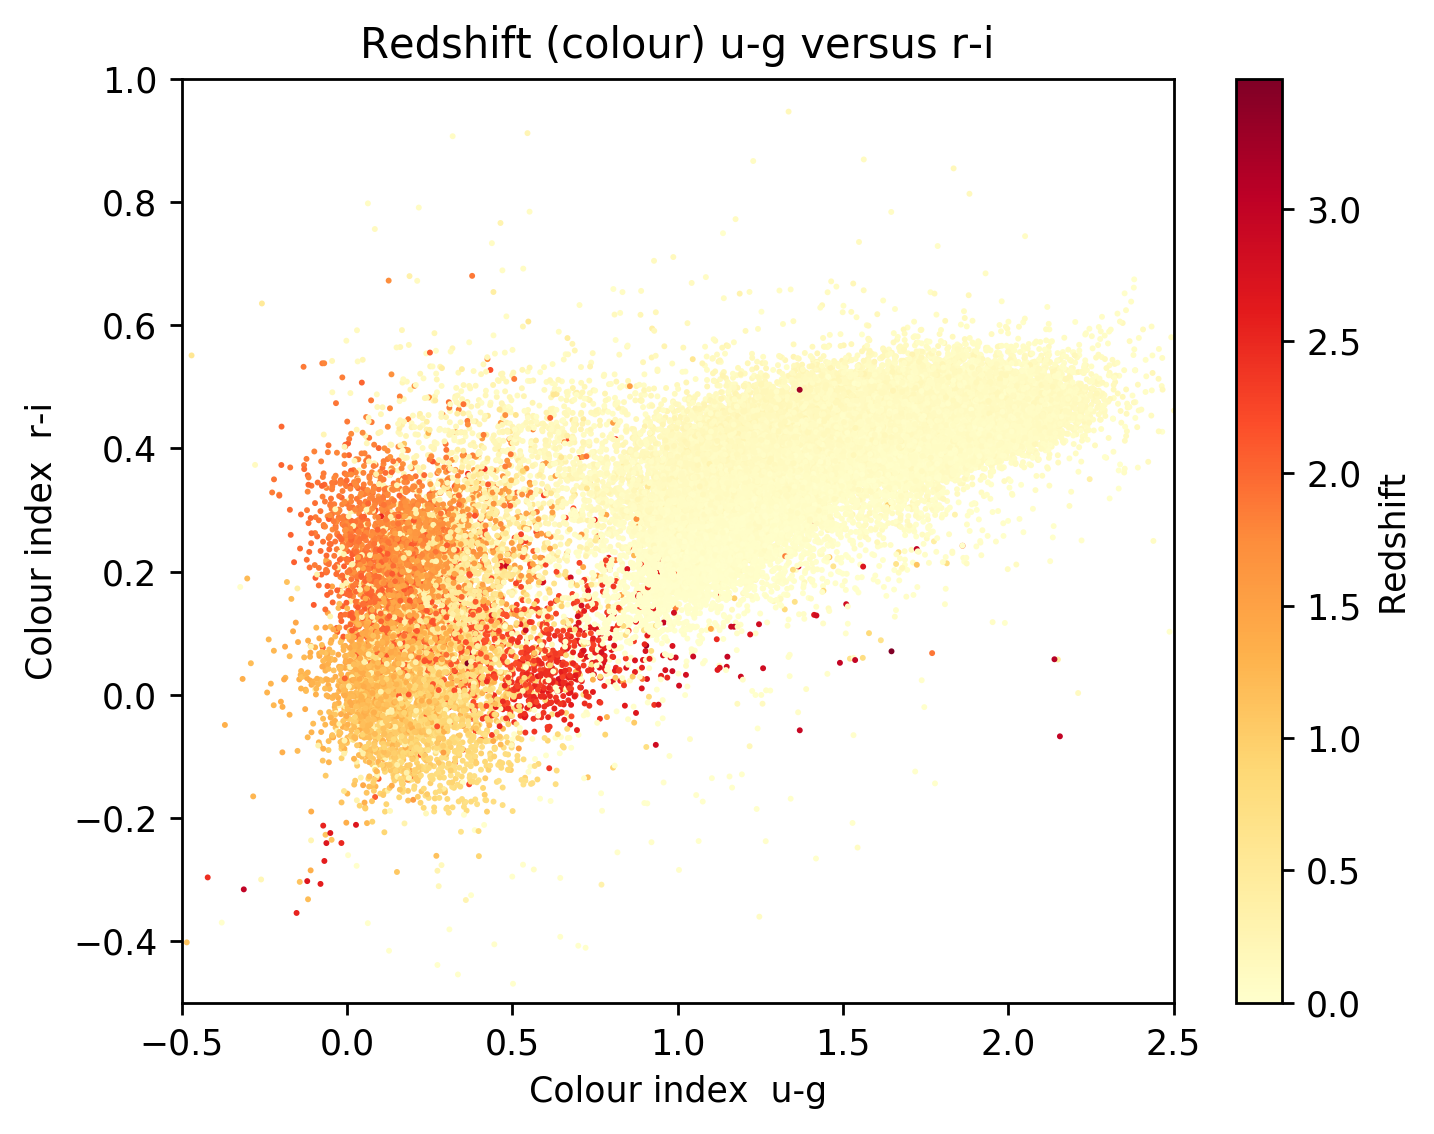
\includegraphics[scale=0.18]{img/redshiftug.png}
        % \caption*{SDSS Data Sample}
    \end{figure}
    \end{frame}
\subsection{Desicion Tree Algorithm}
\begin{frame}
	\frametitle{Detailed overview of Decision Tree}
    \begin{figure}
        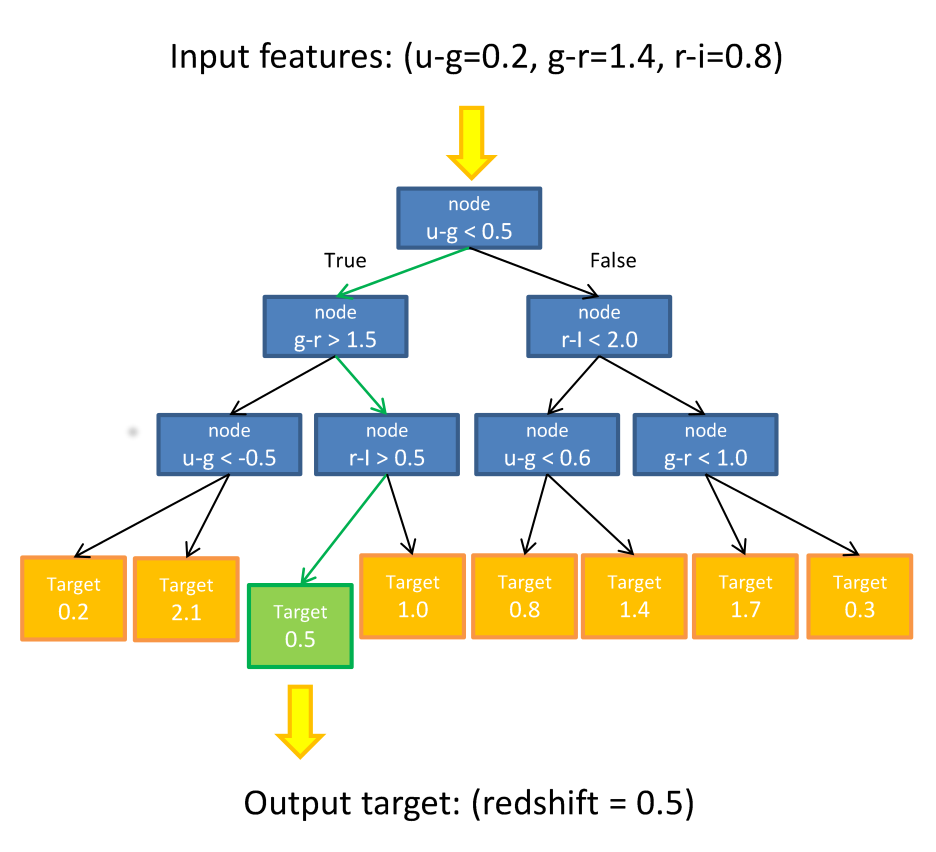
\includegraphics[scale=0.25]{img/decision_tree.png}
        \caption*{Exploring the Output Tree}
    \end{figure}
    \end{frame}


\begin{frame}
	\frametitle{Optimizing process for Decision Tree}
    \begin{figure}
        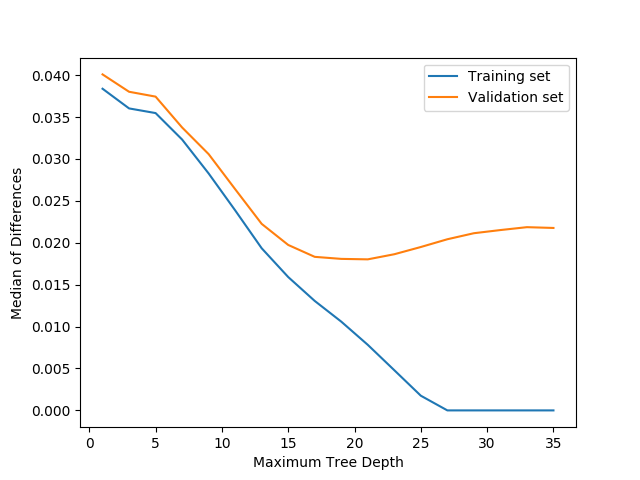
\includegraphics[scale=0.4]{img/overfiting_tree.png}
        \caption*{Setting a Maximum Depth}
    \end{figure}
    \end{frame}
\begin{frame}
	\frametitle{Accuracy of the model}
    \begin{table}[ht]\
        \caption*{The Effect of Training Set Size} % title of Table
        \centering % used for centering table
        \begin{tabular}{c c c c} % centered columns (4 columns)
        \hline\hline %inserts double horizontal lines
        Training Galaxies & Median Diff \\ [0.5ex] % inserts table
        %heading
        \hline % inserts single horizontal line
        50 & 0.048  \\ % inserting body of the table
        500 & 0.026  \\
        5000 & 0.023  \\
        50000 & 0.022  \\ [1ex] % [1ex] adds vertical space
        \hline %inserts single line
        \\
        \end{tabular}
        \label{table:nonlin} % is used to refer this table in the text
        \end{table}
        \begin{equation}
            m e d_{-} d i f f=\operatorname{median}\left(\left|Y_{\mathrm{i}, \text { pred }}-Y_{\mathrm{i}, \mathrm{act}}\right|\right)
            \end{equation}
    \end{frame}
\begin{frame}
	\frametitle{Final Result of Decision Tree Algorithm}
    \begin{figure}
        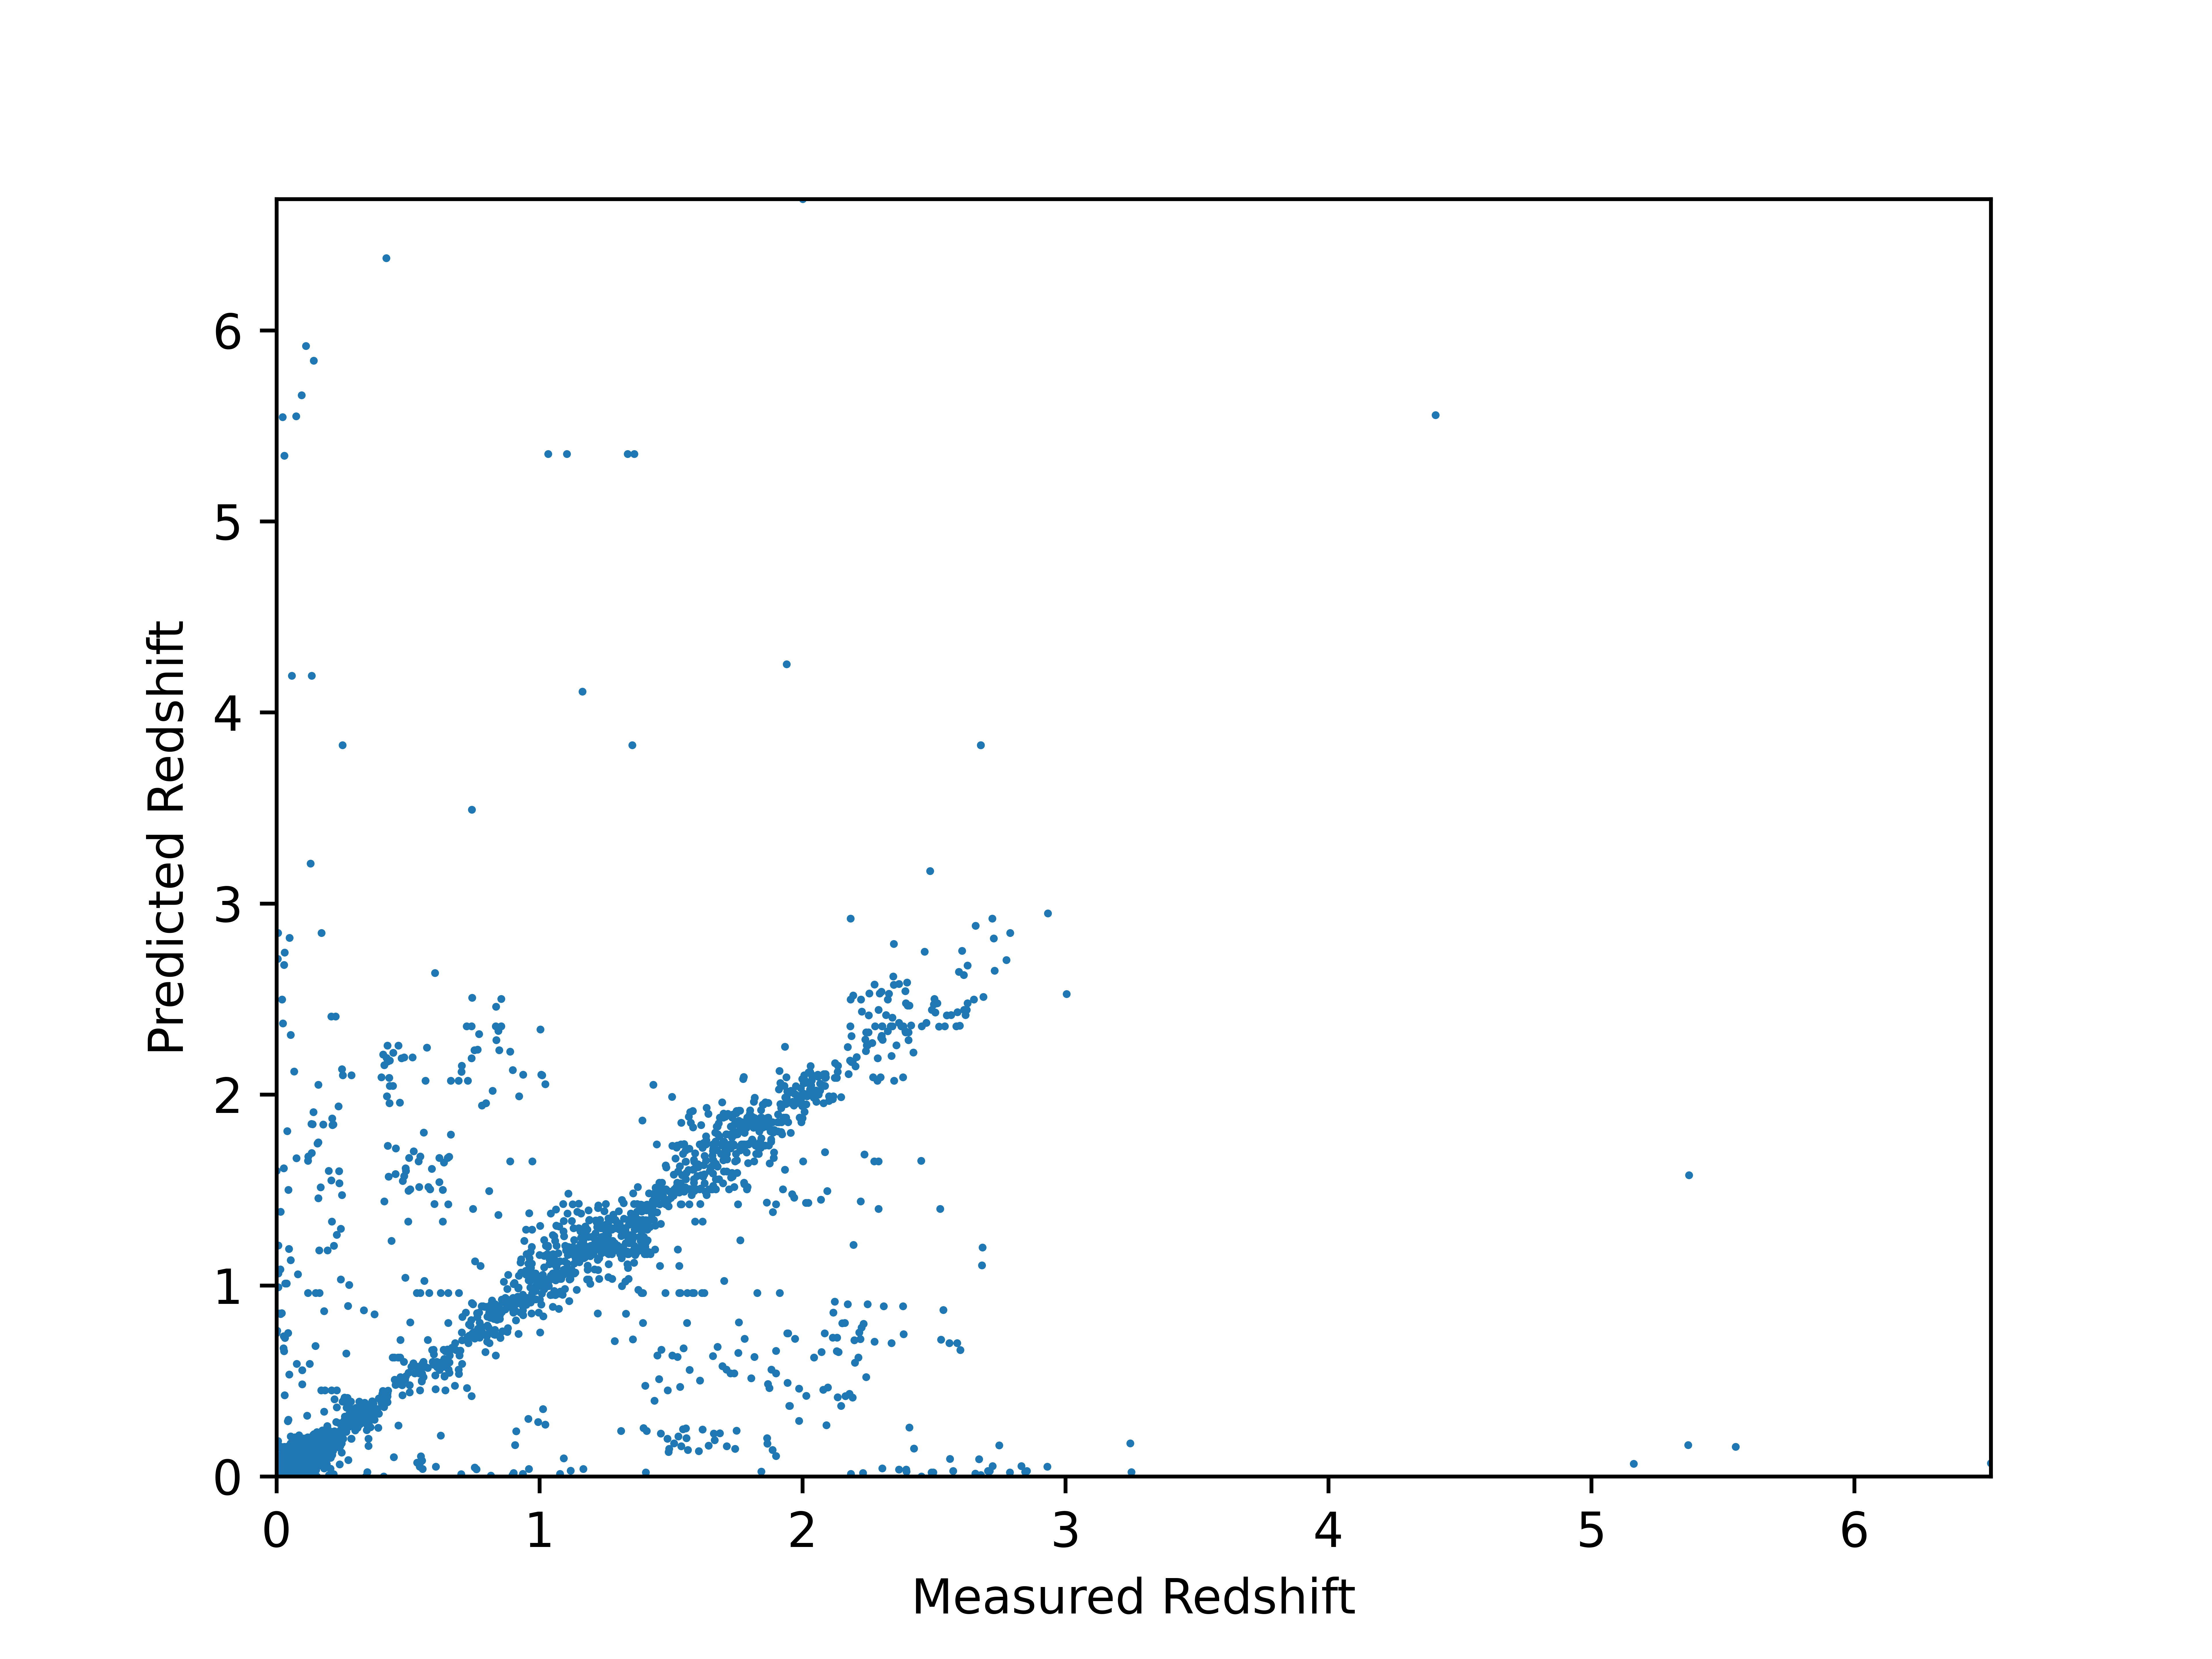
\includegraphics[scale=0.5]{img/Tree_Result.png}
        \caption*{KFold Cross Validated Predictions}
    \end{figure}
    \end{frame}
\subsection{Random Forest Algorithm}
\begin{frame}
	\frametitle{Steps of  preparing Random Forest}
    \begin{columns}[onlytextwidth]
    \begin{column}{.45\textwidth}
        \begin{figure}
            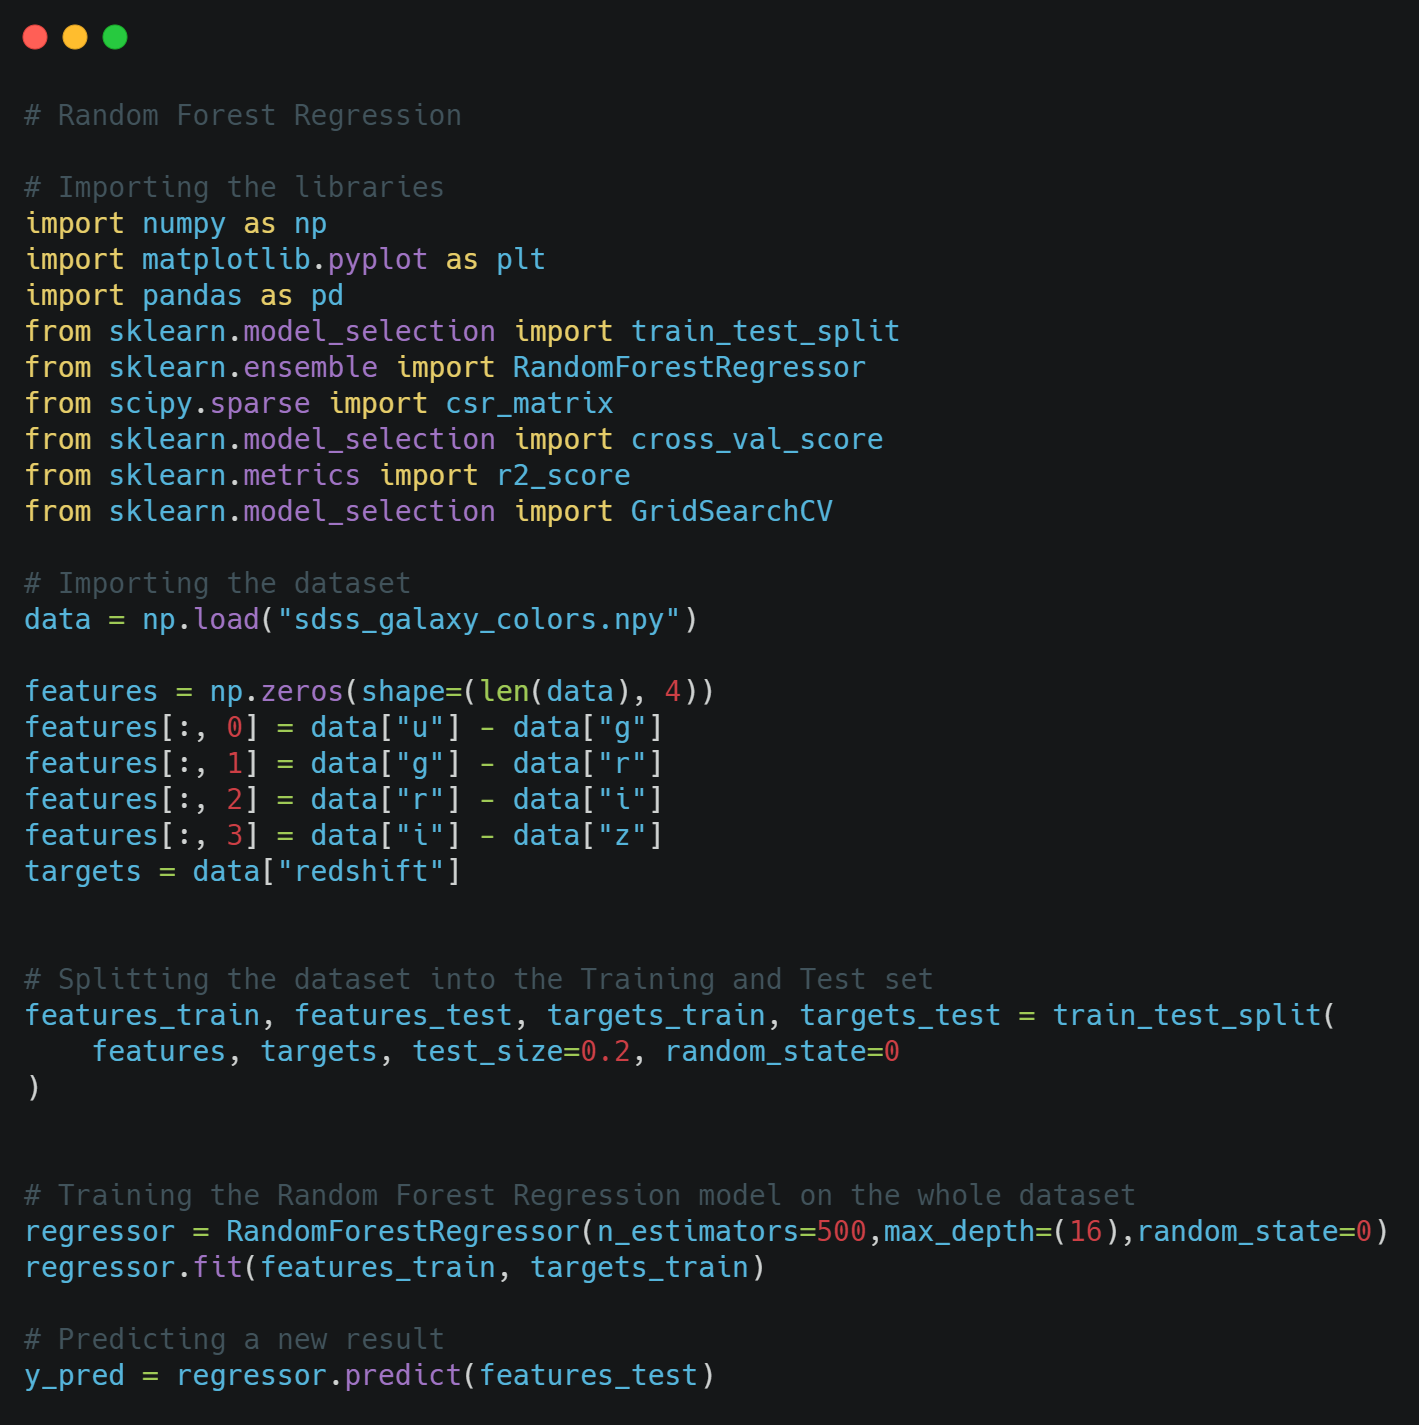
\includegraphics[width=\textwidth]{img/code1-edited.png}
            \caption*{Building a Random Forest Regressor Model}
        \end{figure}
    \end{column}
    \hfill
    \begin{column}{.45\textwidth}
        \begin{figure}
            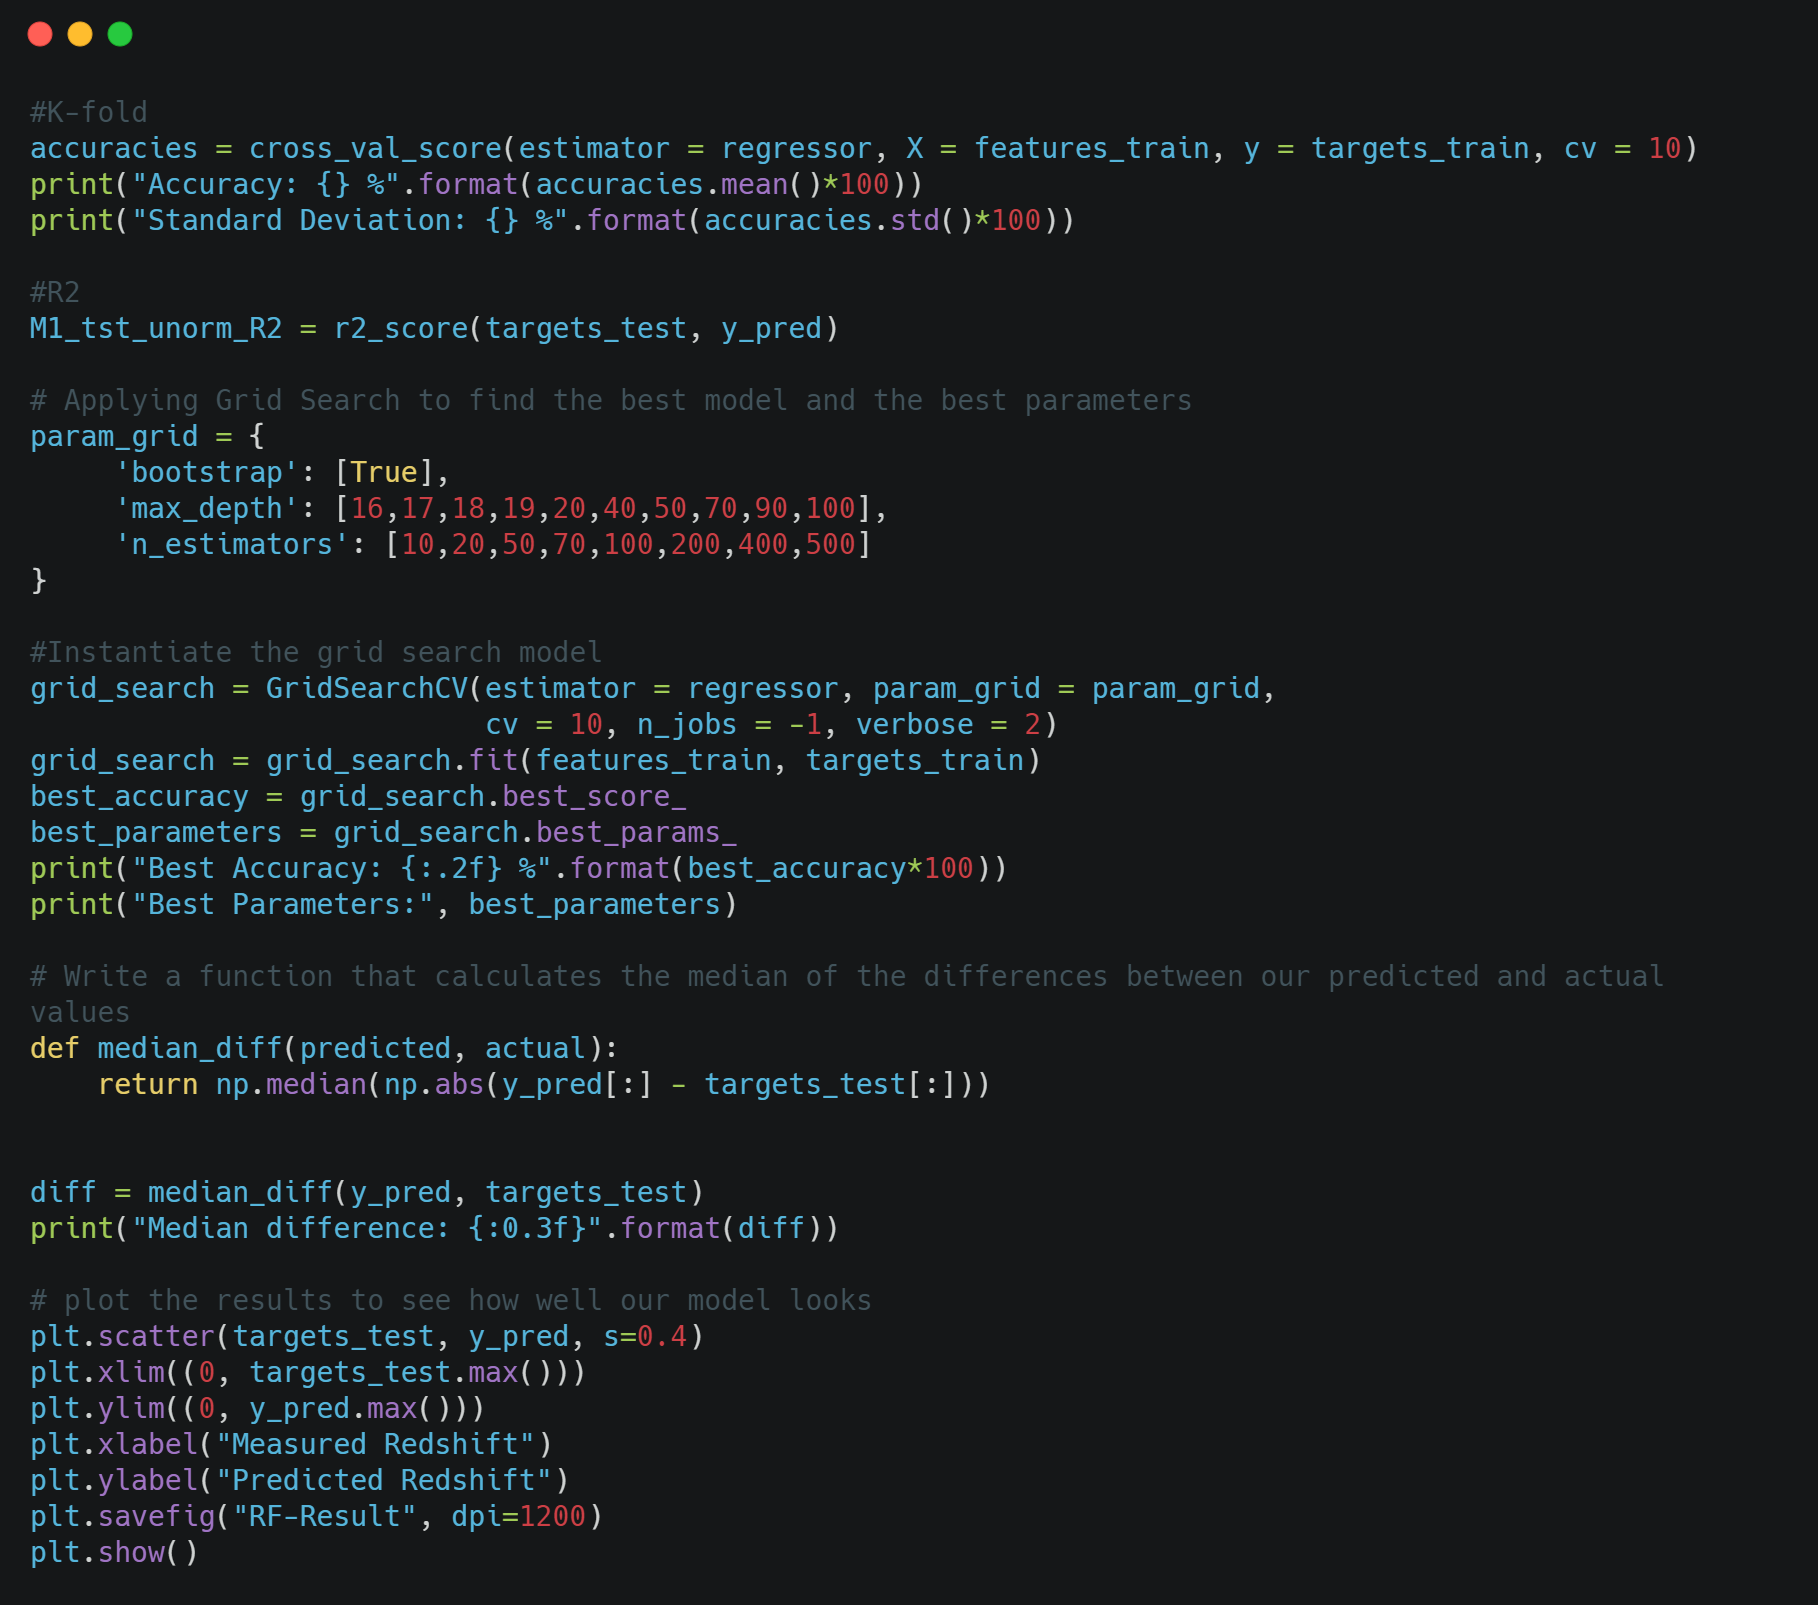
\includegraphics[width=\textwidth]{img/code2-edited.png}
            \caption*{Optimizing the Random Forest Regressor Model}
        \end{figure}
    \end{column}
    \end{columns}
    \end{frame}

\begin{frame}
	\frametitle{Final Result of Random Forest Algorithm}
    \begin{figure}
        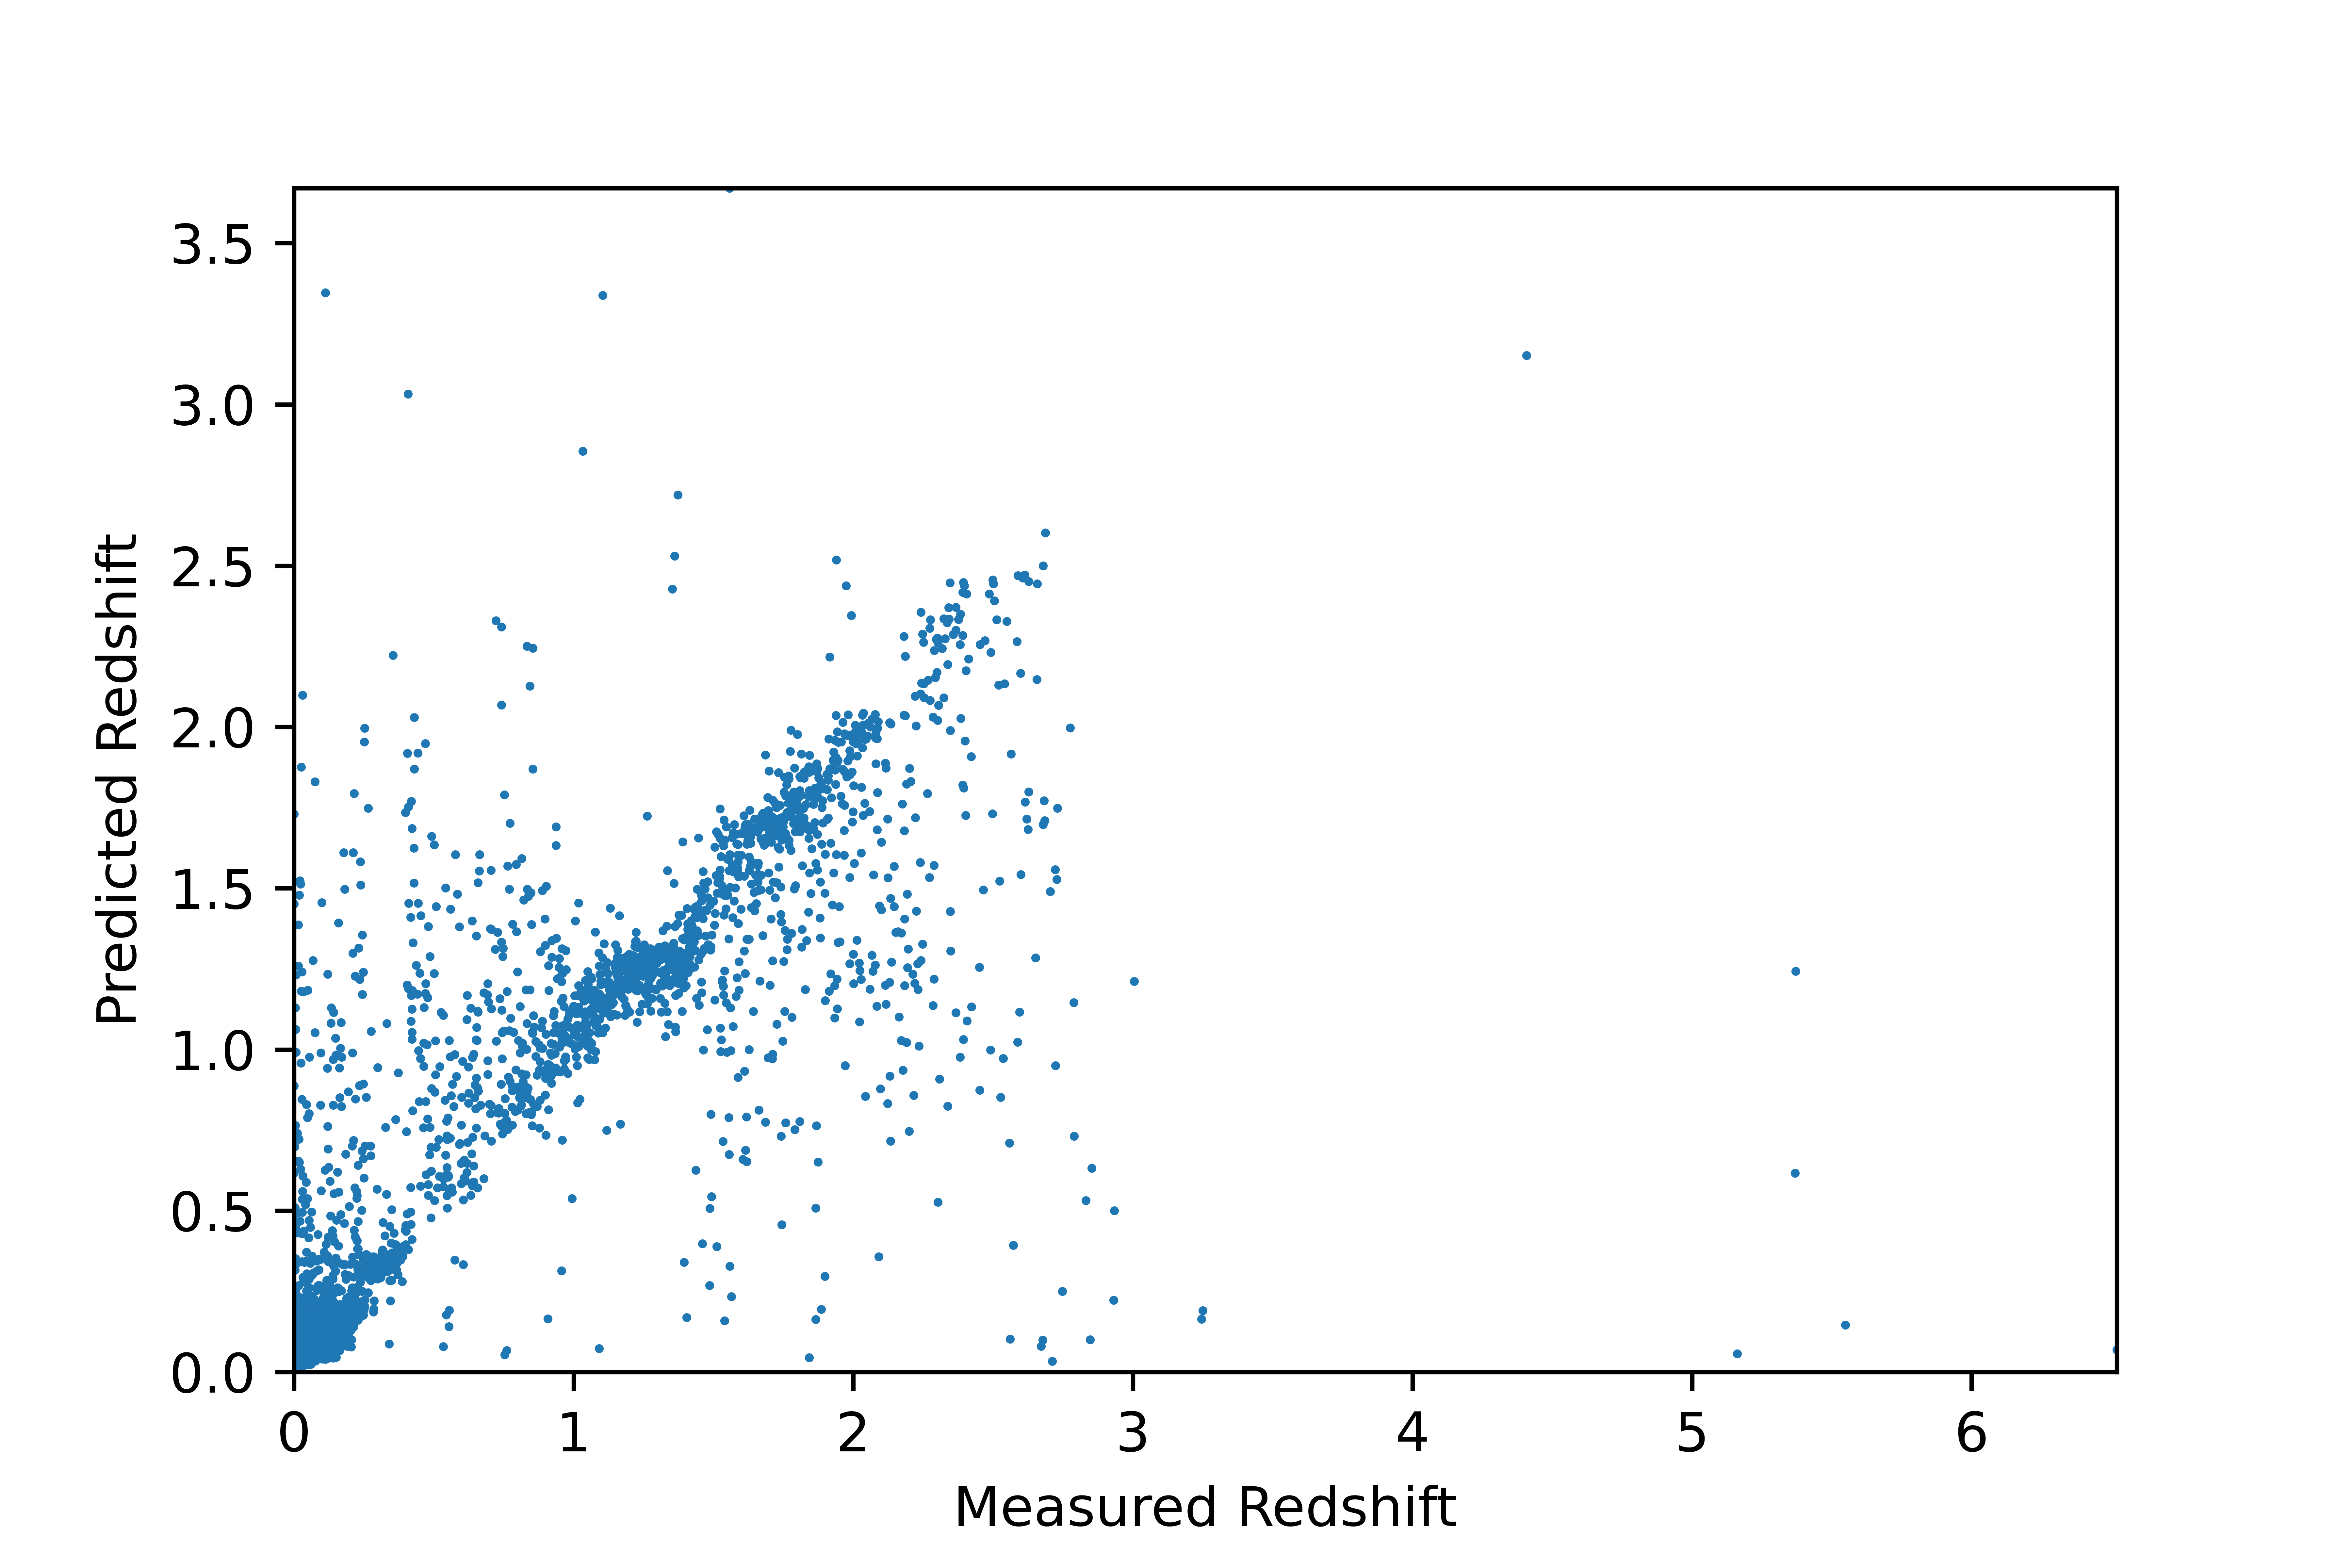
\includegraphics[scale=0.64]{img/RF-Result.png}
        \caption*{KFold Cross Validated Predictions}
    \end{figure}
    \end{frame}

\begin{frame}
	\frametitle{Optimization process}
    \begin{figure}
        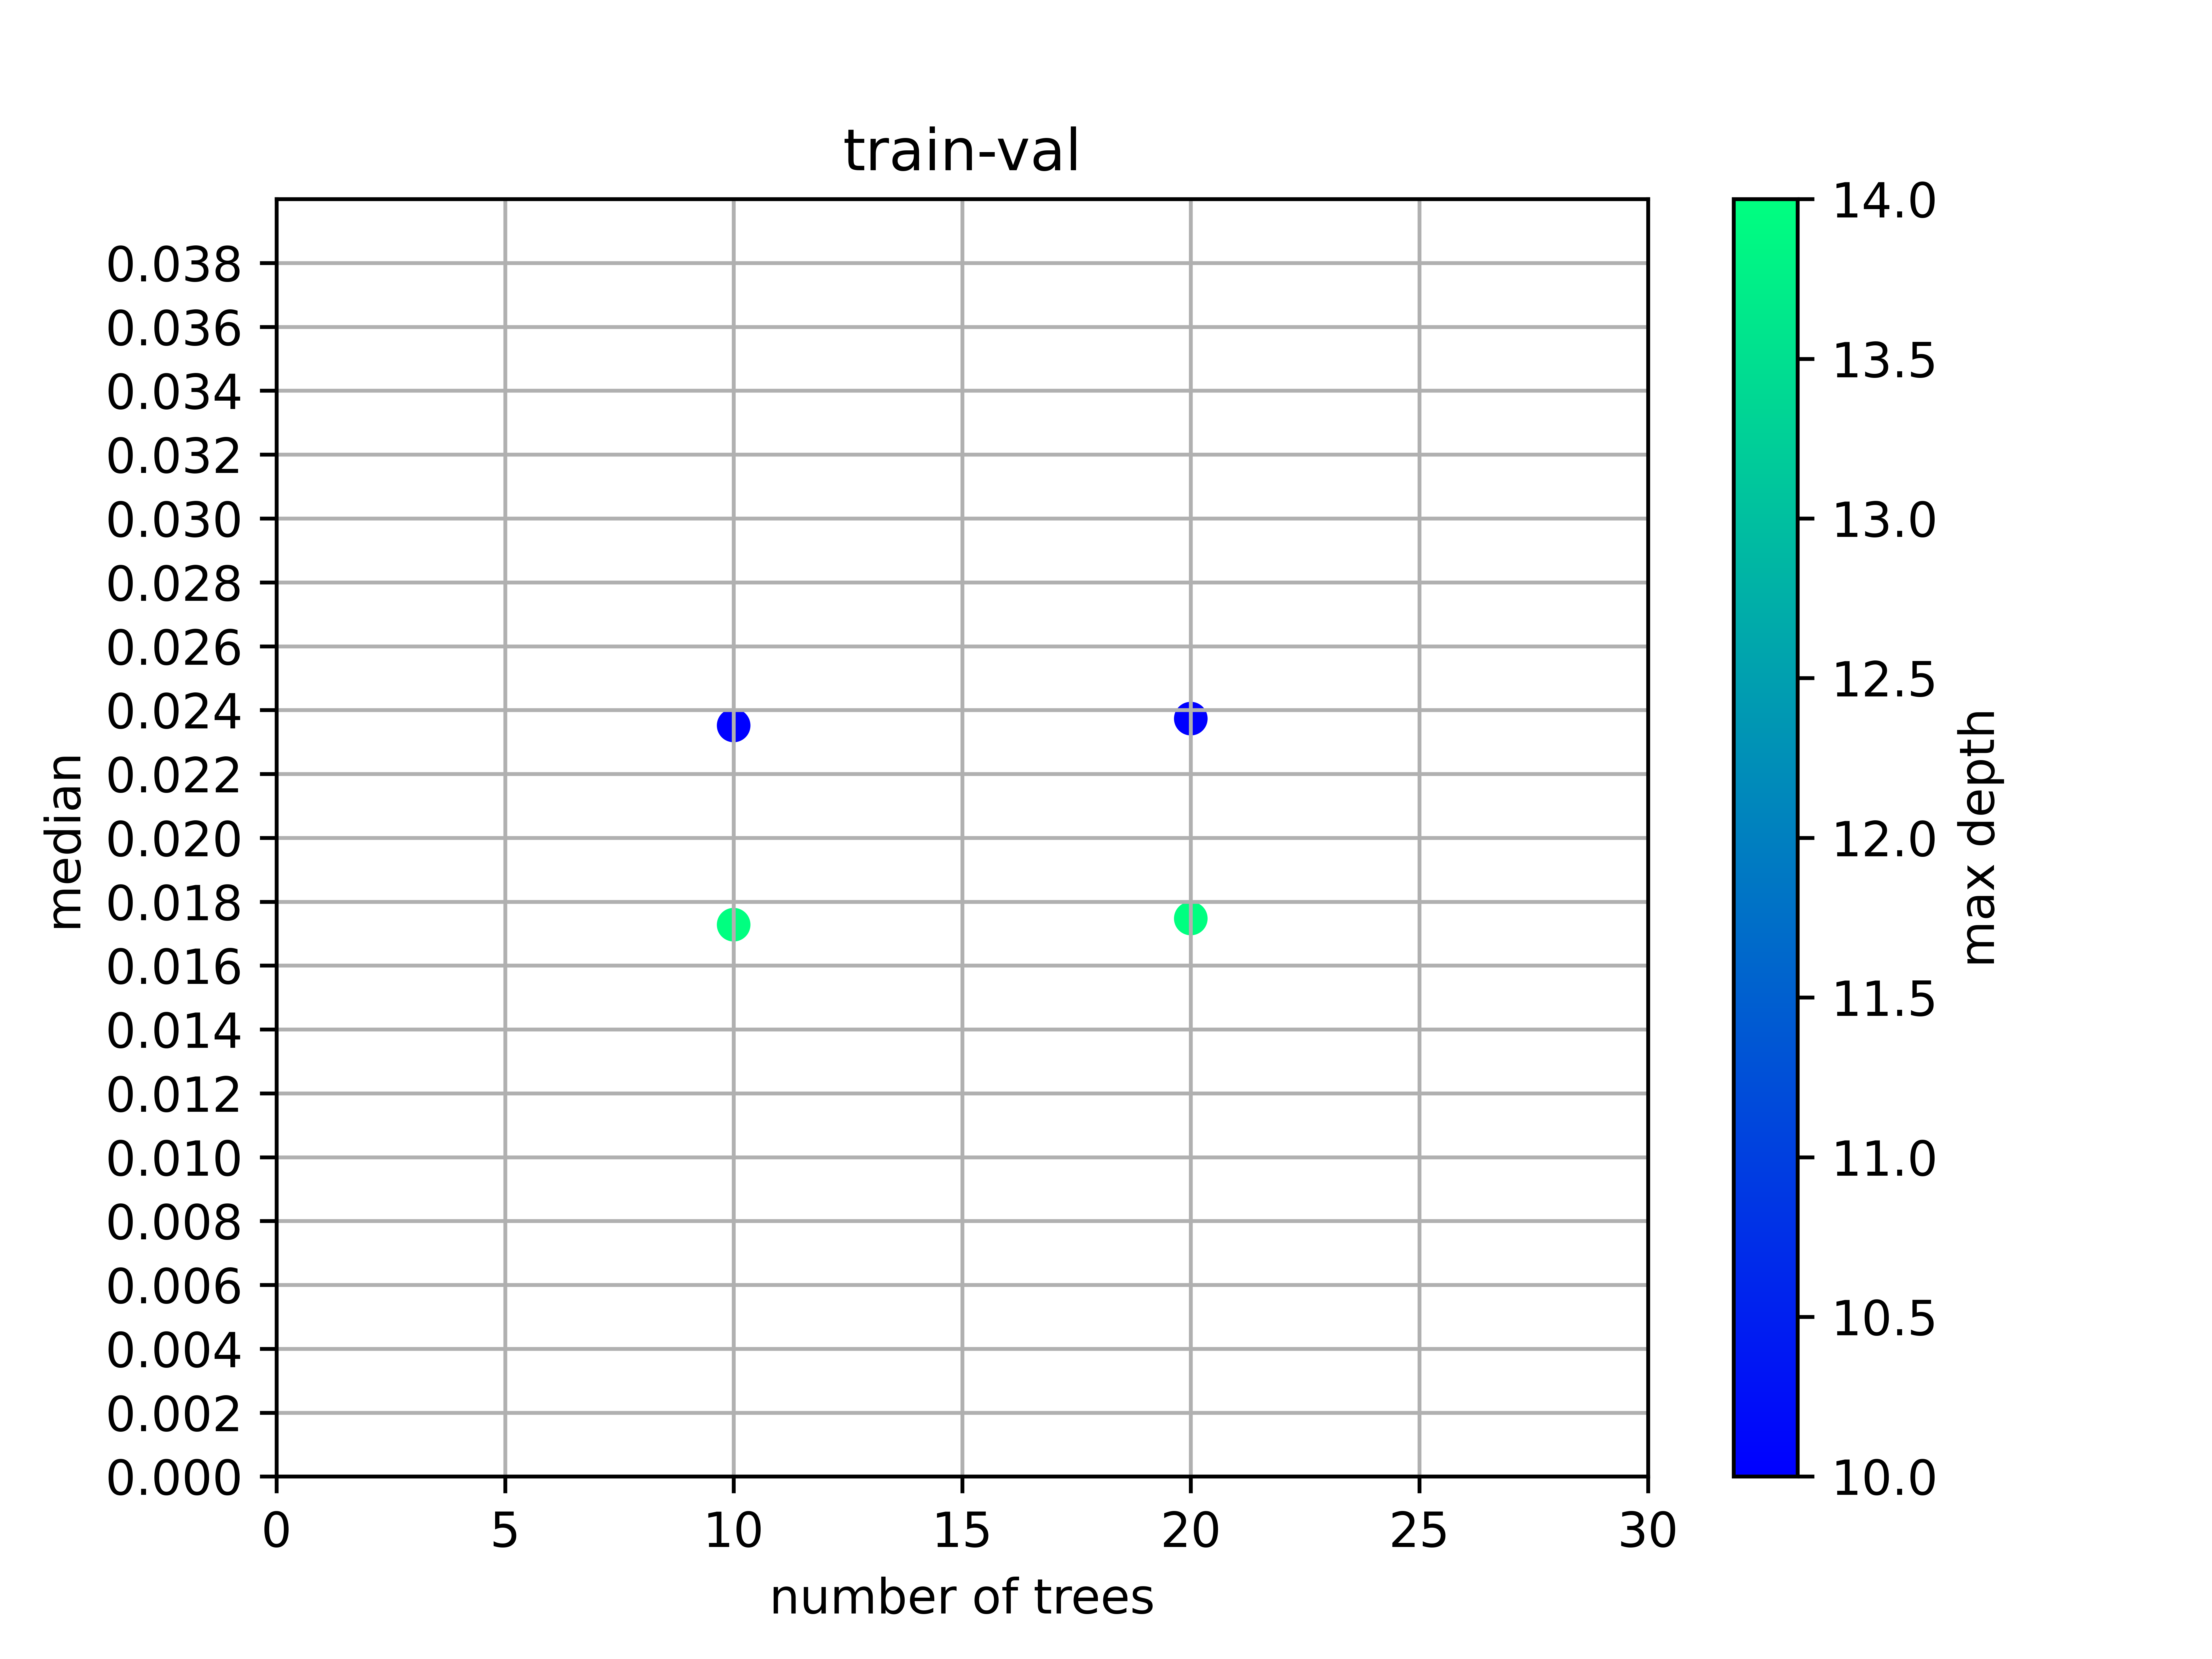
\includegraphics[scale=0.60]{img/train-val.png}
        % \caption*{KFold Cross Validated Predictions}
    \end{figure}
    \end{frame}
\subsection{Validation}
\begin{frame}
	\frametitle{Cross-Validation of two algorithms}
    \begin{figure}
        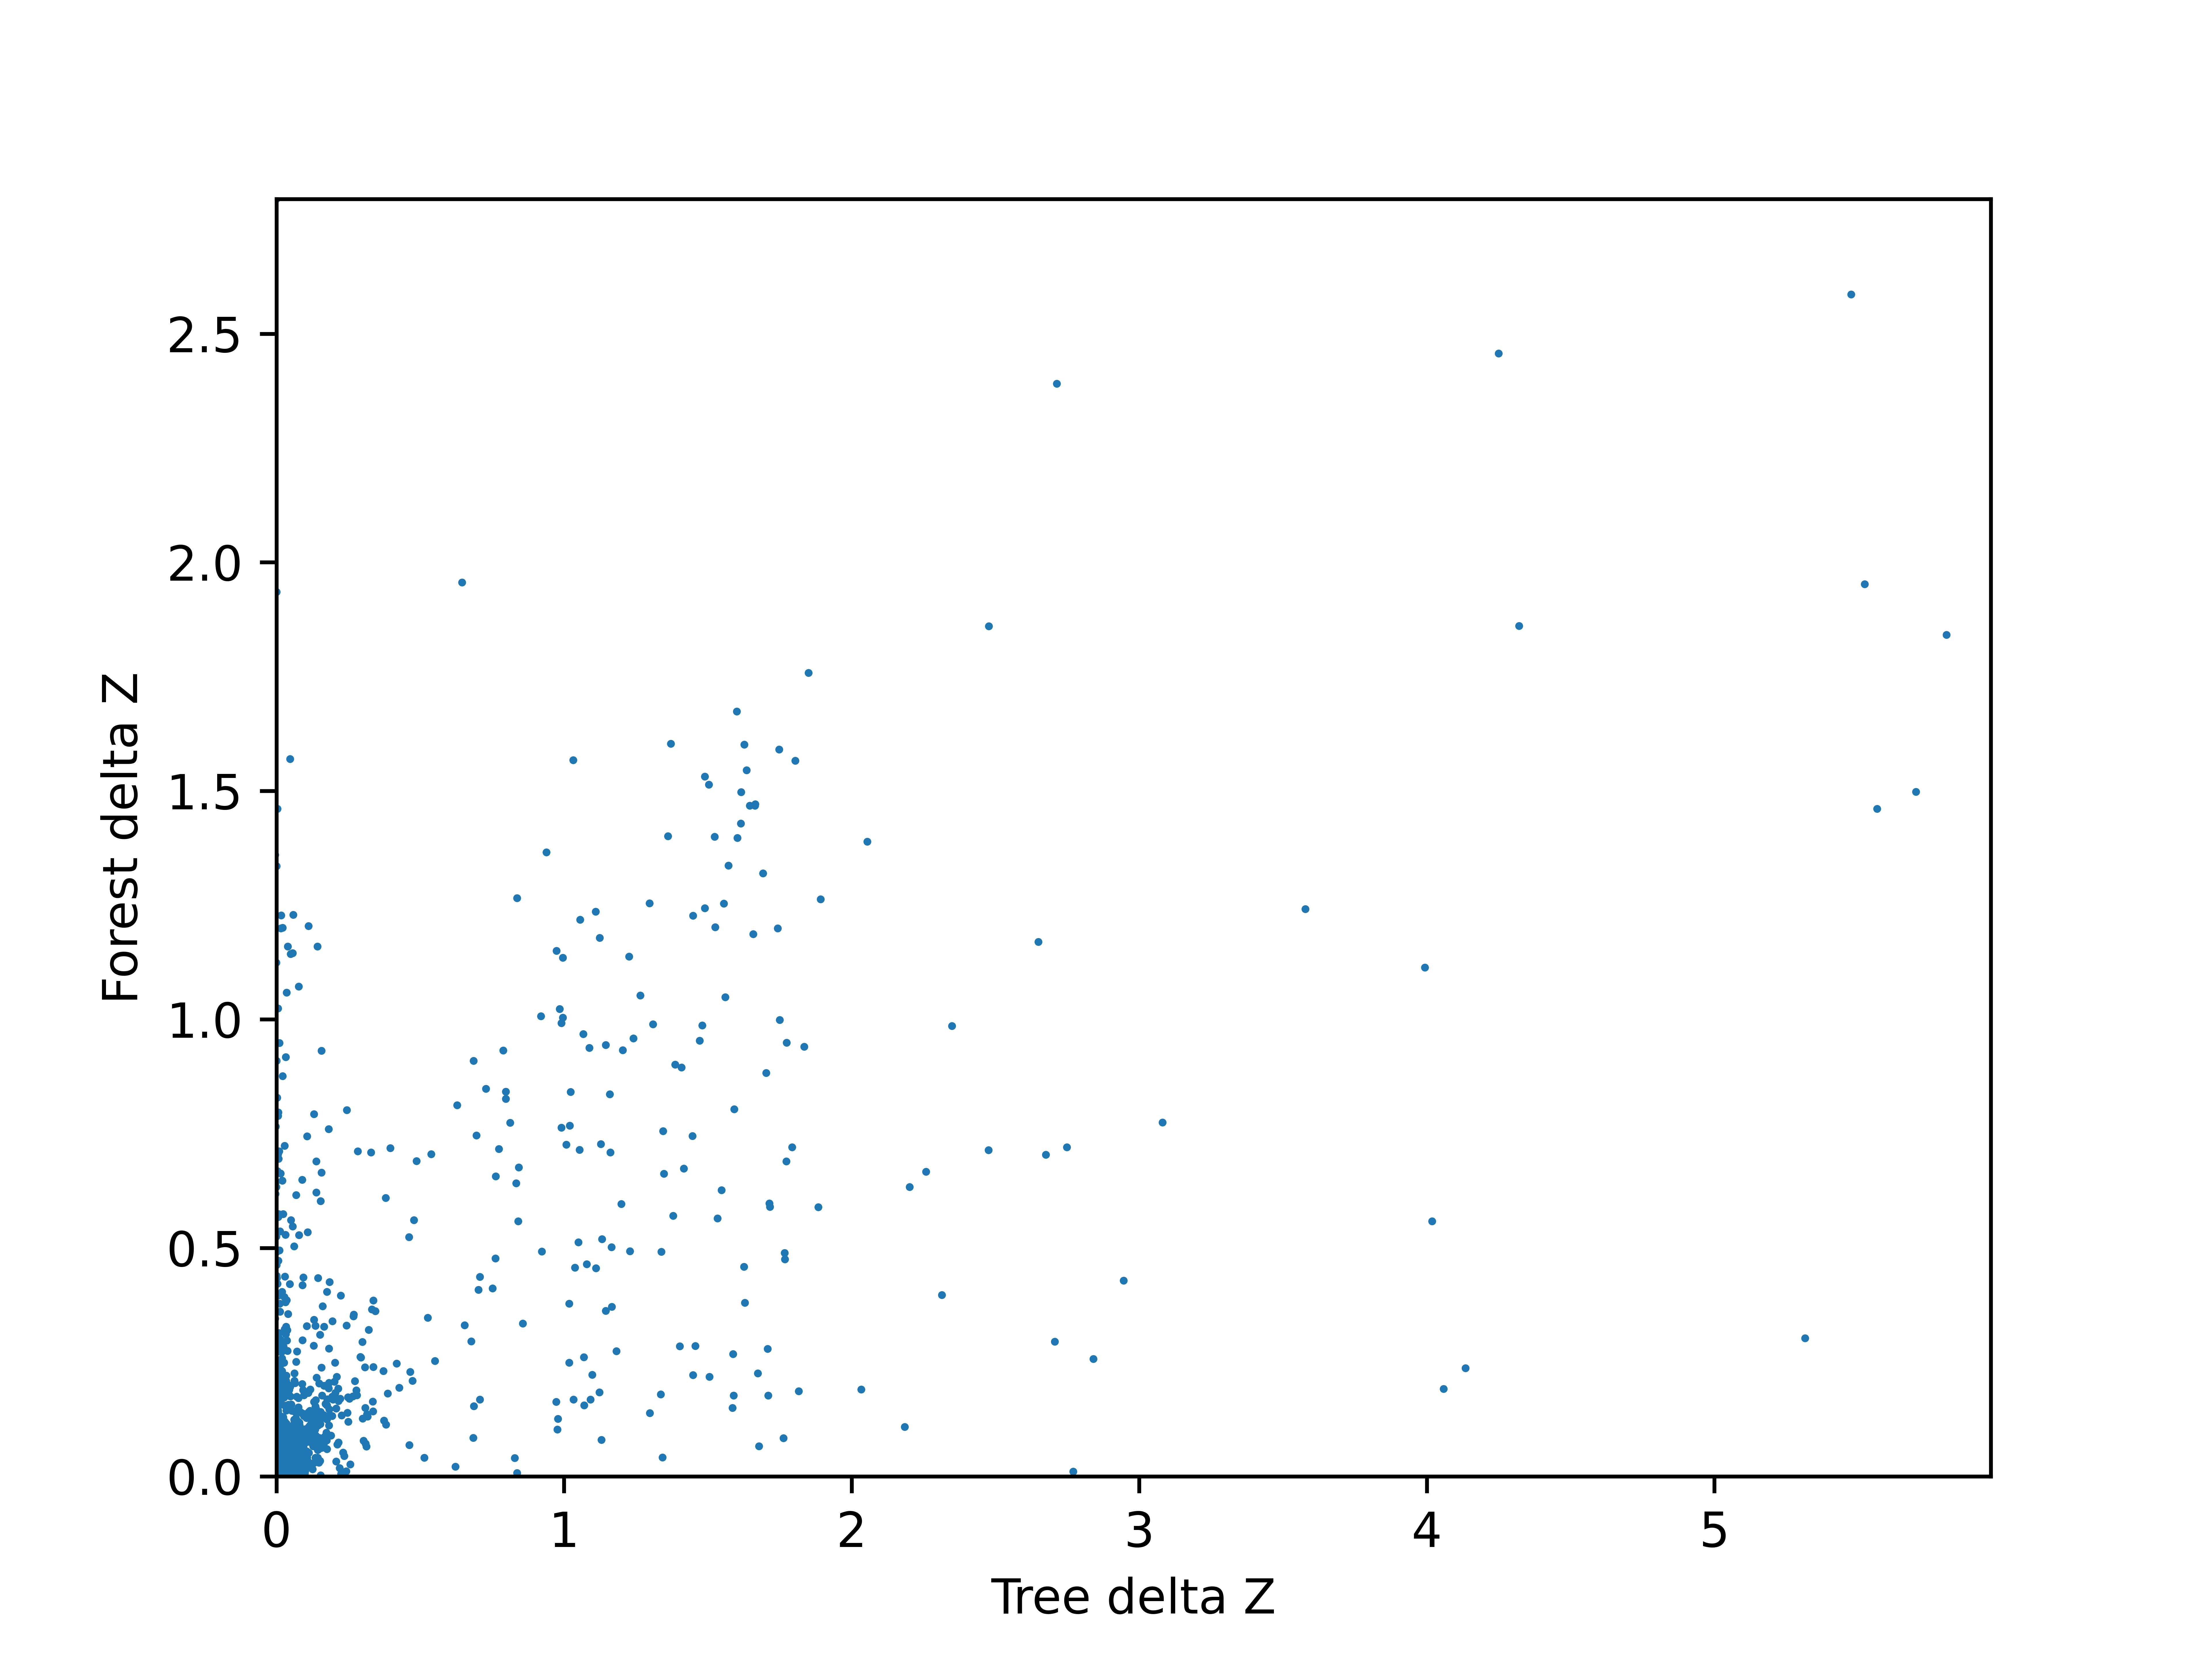
\includegraphics[scale=0.60]{img/deltaZ.png}
        % \caption*{KFold Cross Validated Predictions}
    \end{figure}
    \end{frame}
\begin{frame}
	\frametitle{Analytical Overview}
    \begin{table}[ht]\
        \caption*{Parameters of Regression Modeling} % title of Table
        \centering % used for centering table
        \begin{tabular}{l l l} % centered columns (4 columns)
        \hline\hline %inserts double horizontal lines
         &Decision Tree & Random Forest\\ [0.5ex] % inserts table
        %heading
        \hline % inserts single horizontal line
        Mean Accuracy& 52.19\%  & 73.34\%  \\ % inserting body of the table
        Best Accuracy & 54\% & 76\%  \\
        Max Depth & 19 & 16  \\
        Number of Trees &  1 & 500  \\
        Bootstrap &  True & True  \\
        Standard Deviation &   6.27\% & 2.80\%  \\
        R2 Squared &  0.54 & 0.76  \\
        Median Diff &  0.17 & 0.17  \\ [1ex] % [1ex] adds vertical space
        \hline %inserts single line
        \\
        \end{tabular}
        \end{table}       
        \end{frame}
%----------------------------------------------------------------------------------------
%   Results & Disscusion
%----------------------------------------------------------------------------------------
\section{Results and Disscusion}


%----------------------------------------------------------------------------------------
\begin{frame}
\Huge{\centerline{Thanks For Your Attention :)}}
\end{frame}

%----------------------------------------------------------------------------------------
\end{document} 




% Mean Accuracy & Best Accuracy & Max Depth & Number of Trees & Bootstrap & Standard Deviation & R2 Squared & Median Diff